\bigskip

Dalla modellazione tramite diagrammi UML è possibile passare ad una rappresentazione dei protocolli mediante il Region Connection Calcolus (RCC), in questo caso è stato utilizzato RCC 5.

Il Region Connection Calcolus viene utilizzato per la rappresentazione spaziale qualitativa e per il ragionamento. Le regioni vengono descritte astrattamente in base alle possibili relazioni tra loro.
Come intuibile dal nome RCC 5 consente 5 tipi di relazione tra due regioni:

\begin{figure}[h!] 
    \begin{minipage}{.5\linewidth}
    \centering 
    \subfloat[Equal EQ]{
        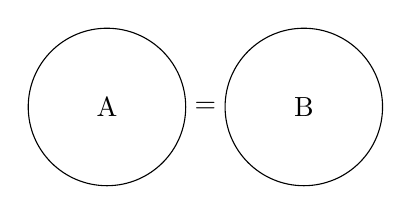
\begin{tikzpicture}[scale=0.5][thick]
            \node at (2.5, 0) {$=$};
            \draw (0,0) circle (2cm);
            \draw (5,0) circle (2cm);
            \draw (0,0) node {A};
            \draw (5,0) node {B};
         \end{tikzpicture} 
    }
    \end{minipage}%
    \begin{minipage}{.5\linewidth}
    \centering
    \subfloat[DiscRete from DR]{
        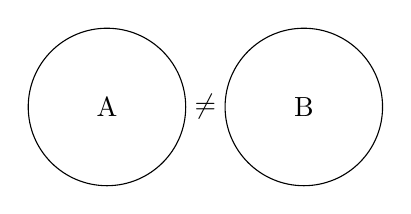
\begin{tikzpicture}[scale=0.5][thick]
            \node at (2.5, 0) {$\neq$};
            \draw (0,0) circle (2cm);
            \draw (5,0) circle (2cm);
            \draw (0,0) node {A};
            \draw (5,0) node {B};
         \end{tikzpicture}
    }
    \end{minipage}%
    \\
    \begin{minipage}{.5\linewidth}
        \centering 
        \subfloat[Proper-Part-of PP]{
            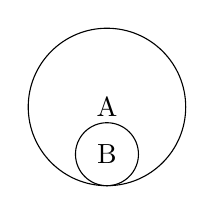
\begin{tikzpicture}[scale=0.5][thick]
                \draw (0,0) circle (2cm);
                \draw (0,-1.2) circle (0.8cm);
                \draw (0,0) node {A};
                \draw (0,-1.2) node {B};
             \end{tikzpicture} 
        }
        \end{minipage}%
        \begin{minipage}{.5\linewidth}
        \centering
        \subfloat[Proper-Part-of-inverse PPi]{
            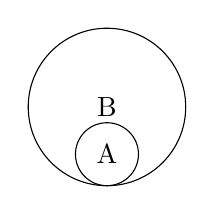
\begin{tikzpicture}[scale=0.5][thick]
                \draw (0,0) circle (2cm);
                \draw (0,-1.2) circle (0.8cm);
                \draw (0,0) node {B};
                \draw (0,-1.2) node {A};
             \end{tikzpicture}
        }
        \end{minipage}%
        \\
        \begin{minipage}{.5\linewidth}
            \centering 
            \subfloat[Partial-Overlap PO]{
                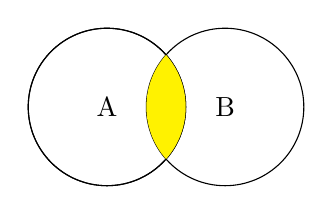
\begin{tikzpicture}[scale=0.5][thick]
                    \draw (0,0) circle (2cm);
                    \draw (3,0) circle (2cm);
                    \draw (0,0) node {A};
                    \draw (3,0) node {B};
                    \draw [clip](0,0) circle (2cm);
                    \fill[yellow] (3,0) circle (2.cm);
                 \end{tikzpicture} 
            }
            \end{minipage}%
    \caption{Possibili relazioni RCC5} 
    \label{fig:rcc5}
\end{figure}

 

%il concetto di regione mereologia e tutto il resto?

%spiegare in cosa consiste, quali operazioni rapperenta, unione, disgiunzione, partial overlap....

%introdurre il concetto di primitiva, come si possono rappresentare mediante rcc 5 